\documentclass[11pt, a4paper, spanish]{article}

%%%%%%%%%% COMIENZO DEL PREAMBULO %%%%%%%%%%

%Info sobre este documento
\author{Jonathan Chiocchio, Gabriel Tursi}
\title{Tesis de Licenciatura Chiocchio - Tursi}

%\usepackage{infostyle}                                                  % provee un look & feel similar a un documento Word
\usepackage[top=2.5cm, bottom=2.5cm, left=2.5cm, right=2.5cm]{geometry}  % m�rgenes
\usepackage[ansinew]{inputenc}                                           % permite que los acentos del estilo ����� salgan joya
\usepackage[spanish, activeacute]{babel}                                 % idioma espa�ol, acentos f�ciles y deletreo de palabras
\usepackage{indentfirst}                                                 % permite indentar un parrafo a mano
\usepackage{caratula}                                                    % incluye caratula est�ndar
\usepackage{graphicx}                                                    % permite insertar gr�ficos
\usepackage{color}                                                       % permite el uso de colores en el documento
\usepackage{url}                                                         % permite el uso de urls
\usepackage[pdfcreator={LaTeX2e},
			pdfauthor={Jonathan Chiocchio, Gabriel Tursi},
			pdftitle={Hacia un modelo m'as flexible para la implementaci'on de la auto reparaci'on de sistemas de software basada en Arquitectura},
			pdfsubject={Hacia un modelo m'as flexible para la implementaci'on de la auto reparaci'on de sistemas de software basada en Arquitectura},
			pdfkeywords={arquitecture design, self-healing, atam, rainbow, ACME},
			pdfstartview=FitH,            % Fits the width of the page to the window
			bookmarksnumbered,            % los bookmarks numerados se ven mejor...
			colorlinks,                   % links con bellos colores
			linkcolor=blue]								% permite cambiar el color de los links
			{hyperref}                    % Permite jugar con algunas cosas que aparecer�n en el PDF final

\selectlanguage{spanish}

\linespread{1.3}                    % interlineado equivalente al 1.5 l�neas de Word...
\pagestyle{myheadings}              % encabezado personalizable con \markboth{}{}
\markboth{}{}												% PONER TITULO PARA ENCABEZADOS DE PAGINAS(el nombre de la tesis es muy largo)
\headsep = 30pt                     % separaci�n entre encabezado y comienzo del p�rrafo

%\addtolength{\oddsidemargin}{-2cm}	% configuracion IDEAL!!!
%\addtolength{\textwidth}{4cm}
%\addtolength{\textheight}{2cm}

% macro 'todo' para To-Do's
\def\todo#1{\textcolor{red}{#1}}

% Macro 'borde' para un texto con borde
\newsavebox{\fmbox}
\newenvironment{borde}[1]
{\begin{lrbox}{\fmbox}\begin{minipage}{#1}}
{\end{minipage}\end{lrbox}\fbox{\usebox{\fmbox}}\\[10pt]}

%%%%%%%%%% FIN DEL PREAMBULO %%%%%%%%%%

\begin{document}

\materia{Tesis de Licenciatura en\\[0.3em]Ciencias de la Computaci�n}
\titulo{Hacia un modelo m'as flexible para la implementaci'on de la auto reparaci'on de sistemas de software basada en Arquitectura}
\integrante{Chiocchio, Jonathan}{849/02}{jchiocchio@gmail.com}
\integrante{Tursi, Germ�n Gabriel}{699/02}{gabrieltursi@gmail.com}
\director{Santiago Ceria}

\maketitle

\thispagestyle{empty}

\newpage

\documentclass[11pt, a4paper, spanish]{article}

%%%%%%%%%% COMIENZO DEL PREAMBULO %%%%%%%%%%

%Info sobre este documento
\author{Jonathan Chiocchio, Gabriel Tursi}
\title{Abstract}

%\usepackage{infostyle}                                                  % provee un look & feel similar a un documento Word
\usepackage[top=2.5cm, bottom=2.5cm, left=2.5cm, right=2.5cm]{geometry}  % m�rgenes
\usepackage[ansinew]{inputenc}                                           % permite que los acentos del estilo ����� salgan joya
\usepackage[spanish, activeacute]{babel}                                 % idioma espa�ol, acentos f�ciles y deletreo de palabras
\usepackage{indentfirst}                                                 % permite indentar un parrafo a mano
\usepackage{caratula}                                                    % incluye caratula est�ndar
\usepackage{graphicx}                                                    % permite insertar gr�ficos
\usepackage{color}                                                       % permite el uso de colores en el documento
\usepackage{url}                                                         % permite el uso de urls
\usepackage{ulem}                                                        % permite el poder tachar texto
\usepackage[pdfcreator={LaTeX2e},
			pdfauthor={Jonathan Chiocchio, Gabriel Tursi},
			pdftitle={Hacia un modelo m'as flexible para la implementaci'on de la auto reparaci'on de sistemas de software basada en Arquitectura},
			pdfsubject={Hacia un modelo m'as flexible para la implementaci'on de la auto reparaci'on de sistemas de software basada en Arquitectura},
			pdfkeywords={arquitecture design, self-healing, atam, rainbow, ACME},
			pdfstartview=FitH,            % Fits the width of the page to the window
			bookmarksnumbered,            % los bookmarks numerados se ven mejor...
			colorlinks,                   % links con bellos colores
			linkcolor=blue]								% permite cambiar el color de los links
			{hyperref}                    % Permite jugar con algunas cosas que aparecer�n en el PDF final

\selectlanguage{spanish}

\linespread{1.3}                    % interlineado equivalente al 1.5 l�neas de Word...
\pagestyle{myheadings}              % encabezado personalizable con \markboth{}{}
\markboth{}{}												% PONER TITULO PARA ENCABEZADOS DE PAGINAS(el nombre de la tesis es muy largo)
\headsep = 30pt                     % separaci�n entre encabezado y comienzo del p�rrafo

%\addtolength{\oddsidemargin}{-2cm}	% configuracion IDEAL!!!
%\addtolength{\textwidth}{4cm}
%\addtolength{\textheight}{2cm}

% macros
\def\todo#1{\textcolor{red}{#1}}
\def\tachar#1{\textcolor{red}{\sout{#1}}}


% Macro 'borde' para un texto con borde
\newsavebox{\fmbox}
\newenvironment{borde}[1]
{\begin{lrbox}{\fmbox}\begin{minipage}{#1}}
{\end{minipage}\end{lrbox}\fbox{\usebox{\fmbox}}\\[10pt]}

%%%%%%%%%% FIN DEL PREAMBULO %%%%%%%%%%

\begin{document}

\normalem                            % Esto impide que el paquete ulem sobreescriba el formateo por defecto del comando ``emph''

\materia{Tesis de Licenciatura en\\[0.3em]Ciencias de la Computaci�n}
\titulo{Hacia un modelo m'as flexible para la implementaci'on de la auto reparaci'on de sistemas de software basada en Arquitectura}
\subtitulo{Resumen extendido}
\integrante{Chiocchio, Jonathan}{849/02}{jchiocchio@gmail.com}
\integrante{Tursi, Germ�n Gabriel}{699/02}{gabrieltursi@gmail.com}
\director{Santiago Ceria}

\maketitle

\thispagestyle{empty}

\newpage

\section{Introducci�n}
		La complejidad creciente de los sistemas desaf�a de forma permanente el estado del arte de las Ciencias de la Computaci�n y la Ingenier�a del Software. La velocidad con la que se producen los cambios, la criticidad de las fallas que aparecen y la necesidad de mantener sistemas funcionando de manera continua a pesar de no pertenecer a lo que tradicionalmente se conoce como ``sistemas de misi�n cr�tica'' ha llevado a los investigadores a buscar novedosas formas de resolver estos desaf�os. Una de ellas es la tendencia hacia los sistemas aut�nomos, que recibe distintos nombres como ``Computaci�n Aut�mona'', ``Software consciente'' o ``Sistemas Auto�Reparables'' (o ``Self Healing'' en ingl�s). Existe una cantidad en aumento de especialistas en el mundo \cite{GAN/03} que creen que esta necesidad de implementar este tipo de mecanismos est� dando lugar al nacimiento de una nueva era en los sistemas de informaci�n.

		La idea subyacente detr�s de estos nombres es que los sistemas incluyan mecanismos para ajustar su comportamiento a partir de fallas o necesidades cambiantes de sus usuarios y/o el entorno en el que operan. De esta forma, un sistema puede repararse u optimizarse sin intervenci�n humana. Una de las formas de implementar estos mecanismos es la llamada ``Adaptaci�n Basada en Arquitecturas''. En este tipo de soluciones, el sistema tiene un m�dulo que conoce su arquitectura, y, en base a este conocimiento y al problema detectado, toma una cierta decisi�n. Uno de los grupos m�s activos en investigaci�n de estos temas es el proyecto \textbf{Rainbow}\cite{Rainbow}, enmarcado dentro del proyecto \textbf{Able}\cite{Able} de la Universidad de Carnegie Mellon (UCM) en Estados Unidos.

La adaptaci�n en Rainbow es lograda a trav�s de varios m�dulos que colaboran para lograr este objetivo. Estos son:

	\begin{itemize}
		\item \textbf{Monitor}: es el m�dulo que se encarga de obtener la informaci�n sobre el funcionamiento del sistema en tiempo de ejecuci�n.
		\item \textbf{Evaluador de Restricciones}: es el que determina si el valor de alguna de las variables que se est�n monitoreando viol� alguna de las restricciones planteadas (por ejemplo, que la \emph{performance} de un proceso dej� de ser aceptable).
		\item \textbf{Modelo de Arquitectura}: es el m�dulo que contiene una representaci�n en un ADL (Architecture Description Language) de la arquitectura del sistema que se quiere adaptar.
		\item \textbf{Manejador de Reparaciones}: es el m�dulo que se ocupa de determinar la forma en la que se va a �reparar� o �adaptar� el sistema en funci�n de los problemas detectados.
		\item \textbf{Int�rprete}: es el m�dulo que interpreta los cambios ocurridos en tiempo de ejecuci�n y los ``traduce'' a cambios en el modelo de arquitectura.
		\item \textbf{Administrador de Runtime}: es el m�dulo que implementa en tiempo de ejecuci�n el cambio en el comportamiento de la aplicaci�n.
	\end{itemize}
	  
		Todos estos mecanismos funcionan de manera externa a la aplicaci�n. Este enfoque tiene varias ventajas, siendo la principal el hecho de contar con un \emph{framework} reusable que pueda ser conectado a distintos tipos de aplicaciones para que implementen mecanismos de adaptaci�n, minimizando el impacto en la aplicaci�n.\\
		El caracter externo de Rainbow representa una ventaja tambi�n cuando se desea implementar auto reparaci�n en sistemas cuyo c�digo fuente no est� disponible o no es plausible de ser modificado.

		A pesar de intentar implementar un mecanismo gen�rico de auto-reparaci�n, Rainbow tiene varios componentes con conocimiento fijo\footnote{M�s conocido com�nmente como ``hardcodeado'' o ``cableado''.} sobre las reparaciones. Por ejemplo, cu�les son las t�cticas para la reparaci�n que se deben implementar cuando una determinada restricci�n es violada.
		
	\subsection{Breve ejemplo de auto-reparaci�n}
		Dado que estos sistemas y sus conceptos son relativamente novedosos, proponemos un peque�o ejemplo de auto-reparaci�n para afirmar conceptos:

		\begin{itemize}
			\item Supongamos una aplicaci�n Web que brinda servicios a millones de usuarios. Es cr�tico que el tiempo de respuesta ante un pedido de una p�gina se mantenga dentro de rangos razonables.
			\item El sistema est� compuesto por varias p�ginas, siendo la m�s cr�tica su p�gina principal. Esta p�gina est� formada por varias ``partes'', cada una con su respectiva funcionalidad.
	    \item El \emph{Monitor} implementa un mecanismo de monitoreo del tiempo de respuesta del sistema ante un pedido, y lo informa al \emph{Int�rprete}, el que a su vez se encarga de traducir dicha informaci�n en cambios en las propiedades del sistema. e.g.\\
	    ``el tiempo de respuesta fue 4.300 ms. $\Rightarrow$ \verb@client.experiencedResponseTime@ $\leftarrow$ \verb@4300@''
	    \item El \emph{Evaluador de Restricciones} determina si las restricciones del sistema siguen cumpliendose o no. Cuando no se respeta el tiempo m�ximo durante una predeterminada cantidad de veces, decide implementar una auto-reparaci�n.
	    \item El \emph{Manejador de Reparaciones}, en funci�n de su conocimiento de la arquitectura del sistema, decide \textbf{desactivar cierta funcionalidad de la p�gina principal}, resignando funcionalidad para ganar en \emph{performance}.
	    \item Ese cambio se implementa a trav�s del \emph{Administrador de Run-Time}.
	    \item  Al desactivar esa funcionalidad, la performance del sistema mejora.
		\end{itemize}
	
\section{Alcance de la tesis}
		La idea de esta tesis es extender el \emph{framework} Rainbow para poder lograr una implementaci�n m�s flexible y poderosa del mecanismo de auto-reparaci�n, ofreciendo a su vez la posibilidad de hacer visible dicho mecanismo a los \emph{stakeholders} de la aplicaci�n, permiti�ndoles involucrarse en la definici�n de escenarios uso real del sistema y su relaci�n con los atributos de calidad requeridos para el mismo; y en la definici�n de prioridades y/o estrategias a considerar en la auto-reparaci�n del sistema.
		
		Esto se pretende lograr con cambios importantes en varios de sus m�dulos:

	\begin{itemize}
		\item Actualmente Rainbow posee conocimiento sobre la arquitectura del sistema a adaptar mediante su modelo de arquitectura (expresado en el ADL Acme\cite{Acme}). Uno de los objetivos de este trabajo es extender dicho conocimiento, para eso, en el m�dulo de \emph{Modelo de Arquitectura}, se implementar�n las siguiente mejoras:
			% BEGIN MEJORAS MODELO ARQUITECTURA -------------------------
			\begin{enumerate}
          \item  Incluir informaci�n sobre los atributos de calidad que la arquitectura implementa y que son relevantes \emph{para el o los stakeholders del sistema} en tiempo de ejecuci�n. Por ejemplo, poder describir la importancia (relativa) de la \emph{performance}, la usabilidad, la disponibilidad, etc.\\
          Nuestro enfoque para lograr esto consiste en especificar  \textbf{Escenarios de Atributos de Calidad} (de ahora en m�s, simplemente ``Escenarios''), un concepto ya especificado por ATAM\cite{ATAM} \cite{ATAM2} (Architecture Tradeoff Analysis Method) en el contexto de los ``Workshops de Atributos de Calidad'' (Quality Attribute Workshops QAW\cite{QAW}).\\
          Un Escenario modela una situaci�n concreta y real de uso del sistema ante la cual el mismo debe comportarse de una manera esperada. Los escenarios est�n compuestos por la siguiente informaci�n:
					\begin{itemize}
		          \item Fuente del Est�mulo
		          \item Est�mulo
							\item Artefacto
		          \item Entorno
		          \item Respuesta
		          \item Cuantificaci�n de la Respuesta
					\end{itemize}
		
					\indent De todos estos atributos, son particularmente importantes el \textbf{Artefacto} y la \textbf{Cuantificaci�n de la Respuesta}.
					
					El \textbf{Artefacto} se refiere al componente, subsistema o parte del sistema afectada por el escenario. Dado que en Acme se especifican los componentes y conectores del sistema, el escenario tendr�a entonces una vinculaci�n directa en la especificaci�n con los componentes afectados.

					La \textbf{Cuantificaci�n de la Respuesta} es tambi�n importante ya que de ella surgen las restricciones que deben ser evaluadas por el \emph{Evaluador de Restricciones}. Al hacer estos cambios, las restricciones que se usaban anteriormente en Rainbow pasar�an a ser en realidad una parte de un Escenario de Atributo de Calidad.
					\item Asignar prioridades a estos escenarios, para que a la hora de escoger una estrategia de auto-reparaci�n, se tengan en consideraci�n otros aspectos del sistema (especificados como atributos de calidad) de modo tal que la estrategia de reparaci�n elegida no comprometa a alguna otra funcionalidad de la aplicaci�n considerada m�s importante para el usuario.
          \item \tachar{Relacionar estos Escenarios (en realidad los artefactos afectados por el escenario) con los modelos de la arquitectura usando la terminolog�a de ATAM\cite{ATAM} (Architecture Tradeoff Analysis Method), para indicar cu�les son los puntos sensibles y los puntos de tradeoff dentro de la arquitectura para los distintos escenarios. De esta manera, el \emph{Manejador de Reparaciones} puede saber d�nde debe cambiar el sistema si un escenario no se est� cumpliendo.}
			\end{enumerate}
			% END MEJORAS MODELO ARQUITECTURA -------------------------

    \item El m�dulo \emph{Evaluador de Restricciones} se extender� para que eval�e la informaci�n de restricciones, presentes en la cuantificaci�n de la respuesta, asociadas a los Escenarios que figuren como activos en el modelo de arquitectura.

    \item En el m�dulo \emph{Manejador de Reparaciones}, utilizar el conocimiento plasmado en los escenarios para optar por la estrategia de reparaci�n a aplicar, teniendo en cuenta los puntos sensibles, los puntos de tradeoff relacionados y las prioridades de los escenarios, con el objetivo de, adem�s de reparar el inconveniente hallado, evitar perjudicar alg�n otro escenario de mayor prioridad.

    \item Una �ltima idea que puede resultar interesante es la de asociar las reparaciones a los escenarios. Por ejemplo, un escenario podr�a incluir informaci�n del estilo ``Si este escenario se ve comprometido, implementar tal reparaci�n''. Esto agrega la ventaja de que ahora los problemas y las soluciones (estrategias), gracias a los escenarios, pueden ser visibles a los usuarios y stakeholders de la aplicaci�n. Dichas estrategias (podr�an ser m�s de una, ordenadas por prioridad al igual que los escenarios) tambi�n deber�an declarar que otros concerns perjudican, para que el \emph{Manejador de Reparaciones} pueda contemplar tradeoffs y decidir la mejor estrategia que no perjudique otros escenarios con dichos concerns.
	\end{itemize}

En resumidas palabras, el alcance del trabajo consiste en:

	\begin{itemize}
    \item Definir las siguientes extensiones:
			\begin{itemize}
          \item Posibilidad de modelar escenarios.
          \item Posibilidad de relacionar escenarios con componentes de la arquitectura.
          \item Posibilidad de especificar \textbf{Puntos Sensibles} y \textbf{Puntos de Tradeoff} en las relaciones entre un escenario y los componentes y conectores que son afectados por �l.
          \item Posibilidad de modelar reparaciones y asociarlas a Escenarios.
			\end{itemize}          
    \item Proponer los cambios en el \emph{Manejador de Reparaciones} y el \emph{Evaluador de Restricciones} de Rainbow, e implementar algunos casos pr�cticos que permitan mostrar c�mo esta estrategia puede funcionar y llevar a un Framework de Adaptaci�n m�s flexible y poderoso. Esto tiene como contrapartida que los usuarios tendr�n m�s control sobre lo que el sistema decida hacer para auto-repararse: s�lo con modificar la informaci�n de los escenarios el sistema modificar� su comportamiento. Por otro lado, las extensiones propuestas en este trabajo hacen que el sistema se comporte de manera m�s aut�noma a medida que se agregan escenarios. Esto parad�jicamente le quita control al usuario, ya que el procedimiento de auto-reparaci�n se vuelve m�s complejo, complicando el seguimiento de las decisiones tomadas por el framework.
	\end{itemize}

\section{Trabajo a futuro}

    Se propone como trabajo a futuro extender la herramienta AcmeStudio para que d� soporte a las extensiones propuestas en el presente trabajo, permitiendo as� modelar escenarios mediante una herramienta gr�fica, lo que ser�a muy �til para stakeholders no t�cnicos. Dicha herramienta es la m�s utilizada hoy en d�a para dise�ar gr�ficamente arquitecturas basadas en el ADL Acme.

\newpage

\begin{thebibliography}{99}
	\bibitem{GAN/03} Ganek, Alan G. y Corbi, Thomas A. The dawning of the autonomic computing era. IBM Syst. J., 42(1):5-18, 2003. ISSN 0018-8670.\\
	\url{http://www.cs.cmu.edu/~garlan/17811/Readings/ganek.pdf}

	\bibitem{Rainbow} Proyecto Rainbow de la Universidad de Carnegie Mellon.\\
	\url{http://www.cs.cmu.edu/~able/research/rainbow/}

	\bibitem{Able} Proyecto Able de la Universidad de Carnegie Mellon.\\
	 \url{http://www.cs.cmu.edu/~able}

	\bibitem{Acme} Proyecto Acme de la Universidad de Carnegie Mellon.\\
	 \url{http://www.cs.cmu.edu/~acme}

	\bibitem{ATAM} ATAM: Method for Architecture Evaluation, Software Engineering Institute (SEI)\\
	 \url{http://www.sei.cmu.edu/library/abstracts/reports/00tr004.cfm}
	 
	\bibitem{ATAM2} The Architecture Tradeoff Analysis Method (ATAM), Software Engineering Institute (SEI)\\
	 \url{http://tinyurl.com/ye5ub9l}

	\bibitem{QAW} Quality Attribute Workshops (QAWs), Third Edition, Software Engineering Institute (SEI)\\
	 \url{http://www.sei.cmu.edu/library/abstracts/reports/03tr016.cfm}

\end{thebibliography}

\end{document}

\newpage

\section{Introducci�n}
	\todo{JONY: mergear con todo lo que pusimos en el abstract en la seccion 2}
	\subsection{Motivaci�n para este trabajo}
		La complejidad creciente de los sistemas desaf�a de forma permanente el estado del arte de las Ciencias de la Computaci�n y la Ingenier�a del Software. La velocidad con la que se producen los cambios, la criticidad de las fallas que aparecen y la necesidad de mantener sistemas funcionando de manera continua a pesar de no pertenecer a lo que tradicionalmente se conoce como ``sistemas de misi�n cr�tica'' ha llevado a los investigadores a buscar novedosas formas de resolver estos desaf�os. Una de ellas es la tendencia hacia los sistemas aut�nomos, que recibe distintos nombres como ``Computaci�n Aut�mona'', ``Software consciente'' o ``Sistemas Auto�Reparables'' (o ``Self Healing'' en ingl�s). Existe una cantidad en aumento de especialistas en el mundo \cite{GAN/03} que creen que la necesidad de implementar este tipo de mecanismos est� dando lugar al nacimiento de una nueva era en los sistemas de software.

		La idea subyacente detr�s de estos nombres es que los sistemas incluyan mecanismos para ajustar su comportamiento a partir de fallas o necesidades cambiantes de sus usuarios y/o el entorno en el que operan. De esta forma, un sistema puede repararse u optimizarse sin intervenci�n humana. Una de las formas de implementar estos mecanismos es la llamada ``Adaptaci�n Basada en Arquitecturas''. En este tipo de soluciones, el sistema tiene un m�dulo que conoce su arquitectura, y, sobre la base de este conocimiento y el problema detectado, toma una decisi�n sobre c�mo auto-repararse.

		Si bien ya existen soluciones de este tipo, en ninguna se considera la participaci�n de los \emph{stakeholders} en el proceso de detecci�n y correcci�n autom�tica de errores. Esto nos motiv� para pensar en qu� manera se los pod�a incluir en el proceso, siempre teniendo en cuenta que su participaci�n deb�a contribuir principalmente en las definiciones de los potenciales problemas y sus posibles soluciones. Esto nos llev� a considerar el uso de los Quality Attribute Scenarios (QAS), los cuales nos permiten definir c�mo deber�a responder el sistema ante determinados est�mulos.
		
		Una vez definidos los escenarios por los \emph{stakeholders}, el paso siguiente consist�a en utilizar toda esa informaci�n en tiempo de ejecuci�n para que el sistema sea capaz de auto-repararse. All� nos servimos de un \emph{framework} de auto-reparaci�n existente llamado Rainbow. Rainbow propone una manera no muy din�mica y muy poco amigable de definir las situaciones en que se deber�a lanzar la auto-reparaci�n, as�, al sumarle los escenarios, se logra mantener todo el potencial de Rainbow y a su vez permitir que los \emph{stakeholders} participen en el proceso de auto-reparaci�n y que tomen conocimiento del dinamismo que podr�a llegar a sufrir el sistema debido a la misma.

	\subsection{Organizaci�n del presente trabajo}
		\todo{JONY: Explicar!}

\newpage

\section{Conclusiones}

	\subsection{Objetivo}

		El presente trabajo permite a los sistemas que implementen Arco Iris \textbf{contar con la definiciones de sus
		requerimientos de atributos de calidad}, en lugar de simplemente poseer implementaciones de posibles soluciones a los
		mismos. No es menor el hecho de que estas definiciones est�n al alcance de todos \emph{stakeholders} participantes,
		cambio radical con respecto al enfoque planteado por Rainbow.

		Este conocimiento es fundamental para lograr el objetivo de esta tesis, que consiste en permitir ampliar el estudio de
		los sistemas aut�nomos introduciendo un modelo flexible de auto reparaci�n basado en la arquitectura de los sistemas,
		ya que adem�s de poner sobre el tablero los requerimientos, los hace visibles a todo el conjunto de participantes del
		desarrollo. De esto se desprende directamente el hecho de que los sistemas podr�n poseer un espectro m�s amplio de
		soluciones, las cu�les ser�n seleccionadas seg�n los requerimientos vayan modific�ndose como consecuencia de
		variaciones en el entorno de ejecuci�n bajo el cual el sistema deba responder. Este dinamismo en la reparaci�n, as�
		como tambi�n la flexibilidad en el modelo de selecci�n de soluciones y su f�cil configuraci�n, hacen de Arco Iris una
		opci�n plausible a ser considerada y extendida para lograr avanzar en la flexibilizaci�n de sistemas inteligentes, a
		la vez que permite incorporar cada vez m�s la utilizaci�n de la auto reparaci�n en la industria del software.

	\subsection{Resumen del trabajo realizado}

		En resumidas palabras, el presente trabajo a�ade una serie de caracter�sticas a Rainbow, todas ellas tendientes a
		disponer de una herramienta gen�rica de auto reparaci�n m�s poderosa y flexible y que, al mismo tiempo, los actores
		funcionales del sistema se vean involucrados en el proceso de definici�n de requerimientos de atributos de calidad,
		puesto que este tipo de actores son los encargados de determinar (junto a arquitectos, dise�adores, etc.) c�mo se debe
		comportar el sistema ante determinadas situaciones de operaci�n. Las caracter�sticas a�adidas en este trabajo son
		b�sicamente las siguientes:
		\begin{itemize}
			\item Posibilidad de modelar escenarios de atributos de calidad siguiendo los principios de ATAM y QAW.
			\item Posibilidad de relacionar escenarios con componentes de la arquitectura.
			\item Posibilidad de especificar prioridades relativas entre escenarios, a ser utilizadas en la elecci�n de la
			estrategia de reparaci�n a ejecutar.
			\item Definici�n de entornos de ejecuci�n para el sistema, con ponderaciones particulares para cada uno
			de los \emph{concerns} existentes, los cuales juegan un papel determinante en el algoritmo de elecci�n de
			estrategias de reparaci�n.
			\item Posibilidad de asociar estrategias de reparaci�n a escenarios.
			\item Modelado de un nuevo algoritmo de elecci�n de la mejor estrategia, utilizando todos los conceptos
			introducidos en Arco Iris.
			\item Implementaci�n de cambios en diversos m�dulos de Rainbow (como por ejemplo, el \emph{RainbowModel} y el
			\emph{AdaptationManager} e implementaci�n de algunos casos pr�cticos que permitan mostrar c�mo esta estrategia
			puede funcionar y llevar a un \emph{framework} de adaptaci�n m�s flexible y poderoso.
			\item Implementaci�n de un mecanismo de recarga din�mica de la configuraci�n de Arco Iris, la cu�l en un futuro
			podr�a ser f�cilmente integrada a Rainbow en pos de dinamizar el uso del \emph{framework}, minimizando su
			\emph{downtime} debido a cambios en la configuraci�n.
			\item Implementaci�n de una herramienta visual de escritorio que permita al usuario de Arco Iris, configurar el
			\emph{framework} de una manera sencilla, amena y eficiente.
		\end{itemize}

		Todo lo antedicho tiene como consecuencia que los usuarios tendr�n m�s herramientas para influir sobre lo que el
		sistema decida hacer para auto repararse: s�lo con modificar la informaci�n de los escenarios el sistema modificar� su
		comportamiento. Como contrapartida, las extensiones propuestas en este trabajo hacen que el sistema se comporte de
		manera m�s aut�noma a medida que se agregan escenarios; esto parad�jicamente le quita control al usuario, ya que el
		procedimiento de auto reparaci�n se vuelve m�s complejo, dificultando el seguimiento de las decisiones tomadas por el
		\emph{framework}.

	\subsection{Arco Iris comparado con Rainbow}

		\noindent En la presente secci�n repasaremos las ventajas que posee Arco Iris por sobre Rainbow. Profundizaremos en
		los siguientes puntos b�sicos:

		\noindent \todo{sacar grafico y poner tabla cuando imprimamos la versi�n definitiva (es para evitar falsos bad boxes)}
%  		\begin{center}
%  			\scriptsize{
%  			\rowcolors*[\hline]{1}{GreenYellow!25}{GreenYellow!10}
%  			\begin{tabularx}{\textwidth}{|X|X|X|X|}
%   			\textbf{Problema} & \textbf{Implementaci�n en Rainbow} & \textbf{Implementaci�n en \mbox{Arco Iris}} &
%   			\textbf{Ventajas}\\
%   			Rapidez en el cambio de configuraci�n & La configuraci�n se lee una vez al principio y no puede ser cambiada
%   			din�micamente mientras Rainbow est� funcionando. & Los escenarios se actualizan din�micamente en \emph{runtime} al
%   			ser modificados. & Una gran parte de los cambios de configuraci�n pasan a impactarse ins\-tan\-t�\-nea\-men\-te,
%   			evitando reiniciar el sistema para cambiar la configuraci�n\\
%   			Informaci�n sobre restricciones & Guardadas en el modelo de la arquitectura (en \mbox{ACME}) & Mediante escenarios
%   			de QAW editados por \emph{stakeholders} & F�cil y transparente agregado y edici�n de las mismas.\\
%   			Decisiones sobre que reparaciones realizar & Tambi�n se encuentran en archivos de configuraci�n & Se evalu�n los
%   			escenarios cargados y como se afectan entre ellos. Luego se invoca a un m�dulo que decide qu� reparaciones pueden
%   			llevarse a cabo en ese contexto. & Posibilidad de extensi�n de dicho m�dulo para inclu�r complejas heur�sticas que
%   			aprendan de los efectos de reparaciones pasadas, etc.\\
%   			Entorno de ejecuci�n (e.g. Alta Carga)& Configurado est�ticamente. Para modificarlo es necesario el reinicio del
%   			\emph{framework}. & Se permite especificar distintos entornos de ejecuci�n. El sistema cambia
%   			di\-n�\-mi\-ca\-men\-te de en\-tor\-no sin necesidad de in\-ter\-ven\-ci�n humana ni reinicio del \emph{framework}.
%   			& Se agrega una nueva variable a considerar para la elecci�n de una estrategia, aumentando la probabilidad de que
%   			la misma se adeque mejor a la situaci�n actual del sistema.
%  			\end{tabularx}
%  			}
%  		\end{center}
			
		\begin{center}
			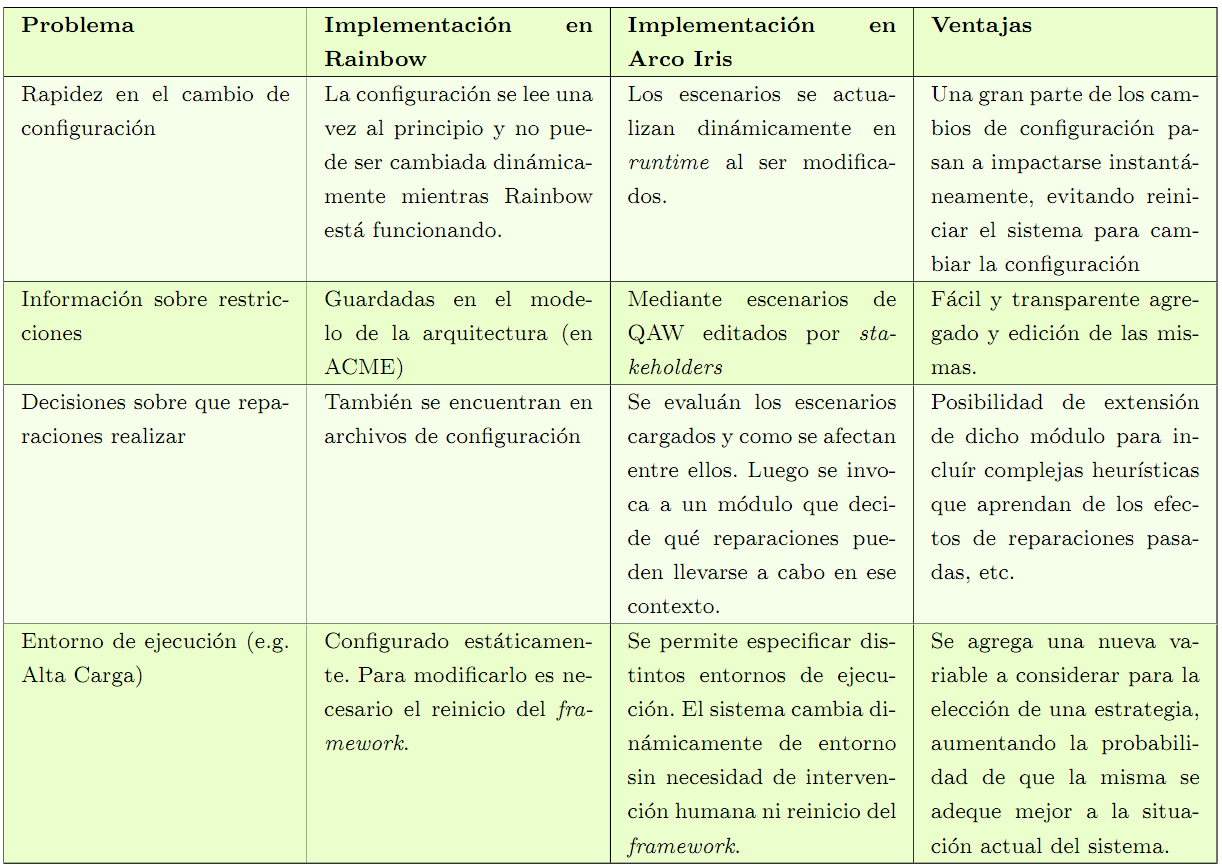
\includegraphics[width=1.00\textwidth]{images/ArcoIrisVsRainbow.png}
		\end{center}

		\subsubsection{Rapidez en el cambio de configuraci�n}
		
			Como se ha mencionado anteriormente, Arco Iris (es decir, Rainbow con las extensiones realizadas en este trabajo)
			trabaja utilizando:
			\begin{itemize}
				\item por un lado, una configuraci�n de \emph{Self Healing} en formato XML, producida ya sea por la herramientas
				Arco Iris UI o bien manualmente; la cual incluye: escenarios de QAW, entornos de ejecuci�n y \emph{artifacts}.
				\item por otro, una bater�a de archivos de configuraci�n heredados de Rainbow, en distintos formatos: stitch, ACME,
				\emph{properties files}, etc.
			\end{itemize}
			Una de las mejoras que agrega este trabajo a Rainbow es el de proveer un mecanismo din�mico de actualizaci�n de la
			configuraci�n de \emph{Self Healing} mediante el cual cualquier modificaci�n en el archivo XML de configuraci�n
			cargada al iniciar Arco Iris, conlleva un ``refresco'' de la configuraci�n que est� siendo usada en tiempo de
			ejecuci�n por el \emph{framework}, sin necesidad de intervenci�n alguna de un operador.
			
			Este dinamismo agregado en lo que respecta a los cambios de configuraci�n, trae aparejado una considerable serie de
			ventajas, a saber:
			\begin{itemize}
				\item ya no es necesario reiniciar el \emph{framework} de auto reparaci�n para modificar cualquier caracter�stica
				relacionada con los escenarios, entornos de ejecuci�n y \emph{artifacts} utilizados en el sistema. Esto evita
				tiempos de no-servicio, recursos involucrados en la reconfiguraci�n y reinicio del sistema, etc. 
				\item se agrega flexibilidad al uso de la herramienta: se podr�an agregar nuevos escenarios, nuevos entornos de
				ejecuci�n que (re)definan situaciones de ejecuci�n concretas, cambiar pesos de \emph{concerns} y/o prioridades relativas
				entre escenarios de acuerdo a necesidades puntuales del negocio e infinidad de otros cambios de configuraci�n
				relevantes a la auto reparaci�n quedar�an impactados en el sistema autom�ticamente.
			\end{itemize}
			
		\subsubsection{Informaci�n sobre restricciones}
		
			Como se ha visto anteriormente, en Rainbow las restricciones impuestas sobre el funcionamiento del sistema (e.g.
			``el tiempo de respuesta para cualquier tipo de \emph{request} no debe superar los 5 m�lisegundos'') son guardadas en
			el modelo de la arquitectura, el cual est� expresado en el lenguaje de descripci�n de arquitecturas \mbox{ACME}.
			Esto claramente representa un impedimento para que los \emph{stakeholders} no t�cnicos puedan participar activamente
			en la definici�n de requerimientos de auto reparaci�n del sistema; ya que de intentarlo, deber�an poder comprender y
			modificar correctamente un diagrama de arquitectura, con sus restricciones escritas en un lenguaje no coloquial sino
			especialmente t�cnico.
			
			En Arco Iris, los \emph{stakeholders} usan una interfaz visual\ref{sec:arcoIrisUI} intuitiva y f�cil de utilizar
			para expresar restricciones del sistema en formato de escenarios de QAW; los cuales a su vez fueron pensados
			originalmente para facilitar la participaci�n de personas con roles funcionales.
			
			La informaci�n incorporada de esta manera, es analizada por Arco Iris para tomar decisiones en tiempo de ejecuci�n
			sobre las auto reparaciones a realizar, considerando una variedad de aspectos, todos ellos configurados en un �nico
			lugar: los escenarios de QAW.
			
			Como vemos, Arco Iris provee una manera simplificada de agregar y/o editar restricciones sobre el sistema, sin
			necesidad de modificar su modelo de arquitectura, sino por medio de los escenarios de QAW. Esto representa una avance
			sobre como funciona Rainbow hoy d�a en ese aspecto.

		\subsubsection{Decisiones sobre que reparaciones realizar}

			Con respecto a este punto, la diferencia principal entre Rainbow y Arco Iris es el enfoque: al momento de
			decidir qu� estrategia es la m�s adecuada para ser ejecutada en el contexto de una o m�s \emph{constraints} no
			cumpliendose, en Rainbow se calcula un \emph{score} para cada una de las estrategias existentes en el sistema,
			mientras Arco Iris busca aquellos escenarios de QAW ``rotos'' y s�lo asigna un \emph{score} a las estrategias
			definidas en dicho subconjunto de escenarios. Este enfoque, adem�s de ser m�s eficiente, es considerablemente mas
			sencillo de configurar y tiene m�s sentido a nivel funcional, ya que en el caso de Rainbow no parece haber una manera
			sencilla de intu�r de antemano qu� estrategia eligir�a en cada caso, hecho que complica en an�lisis de las
			reparaciones efectuadas por Rainbow durante el transcurso de una ejecuci�n.

		\subsubsection{Entorno de ejecuci�n}

			En Rainbow, el concepto de entorno de ejecuci�n es est�ticamente configurado en un archivo de configuraci�n y no se
			modifica de acuerdo al estado din�mico del sistema que se intenta reparar. Para modificar tal est�tico y limitado valor, es
			necesario el reinicio de Rainbow.
			
			El modelo de Arco Iris incluye el concepto de Entorno de Ejecuci�n tal cual es descripto en la
			metodolog�a ATAM\cite{ATAM}, el cual permite al usuario especificar distintos entornos de ejecuci�n posibles para el
			sistema, los cuales poseen restricciones asociadas que se chequean continuamente y que, de cumplirse, hacen que se
			considere que el sistema se encuentra en otro entorno de ejecuci�n, afectando as� al algoritmo de decisi�n de
			estrategias de reparaci�n; ya que dicha decisi�n est� condicionada al \emph{scoring} de estrategias de reparaci�n, el
			cual se realiza considerando los pesos relativos que poseen los \emph{concerns} arquitecturales en el entorno de ejecuci�n
			actual.
			
			Lo antedicho, agrega una nueva arista a las variables consideradas al momento de elegir la mejor estrategia de
			reparaci�n, aumentando las probabilidades de que la estrategia seleccionada sea m�s precisa de acuerdo a la situaci�n
			del sistema en tiempo de ejecuci�n.
			
			Si bien en Rainbow el concepto de ``entorno de ejecuci�n'' no existe como tal, uno podr�a encontrarlo indirectamente
			dentro de ciertas condiciones de aplicabilidad embebidas dentro del c�digo de las estrategias de reparaci�n.
			
			Ahora bien, observemos que Rainbow no tiene forma de determinar a priori si alguna de las estrategias configuradas
			por el usuario van a aplicar en el contexto actual de ejecuci�n: dada alguna \emph{constraint} violada, necesita
			inspeccionar la totalidad de las estrategias para verificar si son aplicables en la situaci�n actual de
			\emph{runtime}. Esto �ltimo es una notable diferencia a favor de Arco Iris, ya que en este caso, al estar las
			estrategias de reparaci�n candidatas embebidas en el escenario, aquellos escenarios cuyo entorno no se corresponda
			con el entorno actual de ejecuci�n, no se considerar�n ``rotos'', evitando c�mputos innecesarios y refinando
			as� el m�todo original provisto por Rainbow.

	\subsection{Compatibilidad hacia atr�s: una empresa sin sentido}

		Uno de los objetivos de dise�o m�s deseables en una extensi�n a un \emph{framework} ya existente como Rainbow, es sin
		dudas que la extensi�n sea ``compatible hacia atr�s'' con \emph{Rainbow}, entendiendose �sto como la capacidad de
		Arco Iris de agregar nuevas caracter�sticas manteniendo al 100\% la funcionalidad original. 
		
		En principio, si se considera �nicamente el dise�o de alto nivel de Rainbow, la idea de una extensi�n \emph{backwards
		compatible} parece factible. Pero, lamentablemente, si se consideran las diferencias conceptuales de ambos modelos,
		no es dif�cil notar que el intento de mantener a ambos conviviendo no s�lo no es una tarea sencilla sino que tambi�n
		carece de sentido, ya que, en algunos puntos claves, son enfoques diametralmente opuestos. Veamos algunos de los
		motivos que apoyan esta idea:
		
		\begin{itemize}
			\item \textbf{C�mo se dispara la auto reparaci�n:} El enfoque de Arco Iris hace centro en el concepto de Escenario
			como medio para expresar requerimientos de atributos de calidad para un sistema. Con lo cual, el inicio de todo el
			proceso de auto reparaci�n se da de una manera sincr�nica con respecto al Est�mulo de alg�n escenario(s) ocurrido en
			el sistema en ejecuci�n. Esto se contrapone con el enfoque de Rainbow, en el cual, peri�dicamente se verifican todas
			las restricciones e invariantes de la arquitectura. Observamos que si quisieramos mantener esta �ltima
			caracter�stica de Rainbow, ya el foco absoluto de la auto reparaci�n no estar�a puesto en los Escenarios de
			atributos de calidad sino que paralelamente existir�an dos flujos distintos de auto reparaci�n disputando entre s�.
			Esto llevar�a a un comportamiento excesivamente complejo y poco predecible, lo cual resulta poco deseable para un
			\emph{framework} de auto reparaci�n.
			\item \textbf{C�mo se decide cu�ndo adaptar:} Arco Iris s�lo intenta efectuar adaptaciones acotadas al escenario o
			los escenarios que se dejan de cumplir en un determinado momento, mientras que Rainbow contempla todo el abanico de
			estrategias disponibles en el caso de que detecte que una violaci�n a una restricci�n o invariante ha tenido lugar.
			Evidentemente, los enfoques son distintos, sin mencionar que los algoritmos de \emph{scoring} de estrategias de
			ambos \emph{frameworks} difieren considerablemente, agregando el algoritmo de Arco Iris nuevas variables a la
			f�rmula, tal como se explica en la secci�n \ref{sec:arcoIrisStrategyScoring}.
		\end{itemize}

	\subsection{Aplicabilidad en sistemas reales}

		Luego de haber repasado las caracter�sticas principales de Arco Iris y de haber entendido su mec�nica, es muy probable
		que al lector se le suscite la siguiente pregunta: �Qu� aplicabilidad tiene esta extensi�n de Rainbow en un	sistema real?
		
		Consideramos que Arco Iris se encuentra un paso m�s cerca de ser utilizado en un sistema de \emph{software} real (i.e.
		en un �mbito no acad�mico) que lo que su antecesor, Rainbow, se encontraba. Esta consideraci�n se basa en el hecho de
		que Arco Iris hace foco en la accesibilidad del usuario final para configurar el \emph{framework} de una manera amena
		y m�s flexible que la provista originalmente por Rainbow, incluyendo una interfaz de usuario visual que facilita dicha
		tarea as� tambi�n como el mantenimiento y evoluci�n de configuraci�n existente.
		
		Habiendo dicho lo anterior, tambi�n reconocemos que Arco Iris todav�a puede no ser la herramienta m�s s�lida y madura
		que los sistemas de \emph{software} de la industria necesitan para confiar la compleja y crucial tarea de agregar auto
		reparaci�n a un sistema. Esto tiene como causas diversos motivos, algunos de los m�s importantes son:
		
		\begin{itemize}
			\item Actualmente, no todas las organizaciones que desarrollan \emph{software} poseen un modelo formal de la
			arquitectura, tal como es requerido por Rainbow o Arco Iris. Esto forma parte de una tendencia por parte de La
			industria del \emph{software} a desarrollar sistemas, a veces de envergadura y de misi�n cr�tica, de una manera
			todav�a artesanal. Esta realidad complica la adopci�n de \emph{frameworks} que centren la auto reparaci�n de un
			sistema en el modelo de su arquitectura. Sin embargo, como hemos mencionado en la secci�n
			\ref{sec:ausenciaObsolescenciaModeloArquitectura}, existen l�neas de investigaci�n intentando atacar este problema,
			derivando el modelo de la arquitectura de un sistema a partir de informaci�n obtenida durante su ejecuci�n, lo cual
			representa un avance importante en pos de facilitar el uso de herramientas como Arco Iris.
			\item El trabajo de creaci�n de \emph{Gauges} y \emph{Probes} (los cuales usualmente no son reutilizables entre
			distintas aplicaciones) sigue siendo una tarea de complejidad no trivial a cargo del usuario del \emph{framework}.
			\item La informaci�n necesaria para que el \emph{framework} funcione, no obstante las mejoras introducidas en Arco
			Iris descritas en la secci�n \ref{sec:actualizacionDinamicaConfig}, sigue estando dispersa en diversos archivos de
			configuraci�n, en archivos separados de estrategias y t�cticas, en el modelo de la arquitectura, etc. Esto, sumado a
			una incompleta documentaci�n de Rainbow, configura una curva de aprendizaje del \emph{framework} un tanto pronunciada
			para un usuario nuevo. Es necesario seguir trabajando en la centralizaci�n de la configuraci�n (tal cual fue descrito
			en la secci�n \ref{sec:todaLaConfigEnUnSoloArchivo}) y tambi�n en el incremento de la documentaci�n para facilitar el
			uso, tanto de Rainbow como de Arco Iris.
		\end{itemize}


\newpage

%	Las citas bibliogr�ficas deber�n ser adecuadas al tema y usando el siguiente formato por orden alfab�tico:
%	[AUT/ZZ] Autores, titulo, Publicaci�n, Editorial, A�o.
\def\refname{Bibliograf�a}

\begin{thebibliography}{99}
	\bibitem{GAN/03} Ganek, Alan G. y Corbi, Thomas A. The dawning of the autonomic computing era. IBM Syst. J., 42(1):5-18, 2003. ISSN 0018-8670.\\
	\url{http://www.cs.cmu.edu/~garlan/17811/Readings/ganek.pdf}

	\bibitem[GIO/82]{GIO/82} Gioan A. ``Regularized Minimization Under Weaker Hypotheses'', applied Mathematics Optimization, Springer Verlag, Volumen 8 numero1 - pag 59-68.1982.

	\bibitem[GMW99]{GMW99} Garlan, D., Monroe R. T., Wile D. \href{http://www.cs.cmu.edu/afs/cs/project/able/ftp/acme-fcbs/acme-fcbs.pdf}{``Acme: Architectural Description of Component-Based Systems''}.

	\bibitem{Scenarios} Kazman, Rick and Abowd, Gregory and Bass, Len and Clements, Paul, Scenario-Based Analysis of Software Architecture, IEEE Computer Society Press, 1996, Los Alamitos, CA, USA. Disponible on-line:\\
	\url{http://eprints.kfupm.edu.sa/63611/1/63611.pdf}
	
	\bibitem{AcmeStudio} Acme Studio Tool, Software Engineering Institute (SEI)\\
	 \url{http://www.cs.cmu.edu/~acme/AcmeStudio/}

	\bibitem{Eclipse} Eclipse Platform\\
	 \url{http://www.eclipse.org/}
	 
\end{thebibliography}

\todo{ver svn/doc}\\
\todo{Libros de Arquitecturas (Ver biblio de IS2)}\\
\todo{Art�culos del SEI de ATAM y QAW}\\
\todo{Tesis de Owen Chen}\\
\todo{Todos los art�culos que nos pas� Garlan sobre Self Healing}\\
\todo{Tesis del flaco de la UCA}

\end{document}